\chapter{Implementación}

En esta sección se describen las etapas llevadas a cabo durante el proceso de la implementación del proyecto, los desafíos encontrados y las soluciones adoptadas. También se incluyen ejemplos de código y capturas de pantalla que ilustran el profreso y los resultados obtenidos.

\section{Preparación del Entorno de Desarrollo}

Antes de iniciar la implementación, se realizó la configuración del entorno de desarrollo. Esto incluyó la instalación de todas las dependencias necesarias y la configuración de herramientas de desarrollo mencionadas en el apartado previo, como Visual Studio Code y Postman.


\section{Servidor}

En este apartado, se describe la implementación en el lado del servidor de la aplicación. Se definirá cómo se realizó la estructura del código y su implementación, proporcionando algunos ejemplos para la creación de la API. A continuación, se definirán los pasos seguidos para lograr esta implementación.

\begin{enumerate}
    \item \textbf{Definición de los Endpoints: }Se definieron los endpoints necesarios para gestionar las llamadas relacionadas con la administración de usuarios, establecimientos, eventos, ofertas y reseñas.

    \item \textbf{Implementación del Modelo: } En esta etapa se implementaron las clases necesarias a partir del diagrama UML del capítulo anterior. Estas clases se encargan de gestionar la comunicación con la base de datos y proporcionar una estructura clara y manejable para los datos utilizados en la aplicación.

    \item \textbf{Implementación de Esquemas: } Se implementaron esquemas para la correcta validación de los datos enviados a la API. Para cada entidad se creó un archivo de esquema específico, lo cual organiza mejor el código y asegura que los datos recibidos cumplan con los requisitos esperados. Esta estructuración facilita la gestión y validación de datos, asegurando la integridad y la consistencia.

    \item \textbf{Implementación de los Endpoints: } La implementación de los endpoints se realizó siguiendo una estructura RESTful. Para cada entidad se creó un archivo de servicio y un bluepring, lo cual evita la repetición de definiciones para cada endpoint. Esta estructura modular garantiza una comunicación eficiente y coherente. La organización del código mediante blueprints además facilita la futura escalabilidad de la API.

    \item \textbf{Pruebas en Postman: } Se realizaron diferentes pruebas para comprobar el correcto funcionamiento de todos los endpoints utilizando la herramienta descrita anteriormente, Postman. Se verificaron las llamadas POST para inserciones a la base de datos, las llamadas GET para obtener información, las llamadas PUT para la modificación de datos y las llamadas DELETE para eliminarlos.
\end{enumerate}

\subsection{Servicios}

El servidor atiende principalmente las solicitudes de creación, consulta, modificación y eliminación de entidades. Estas operaciones pueden ser llevadas a cabo por usuarios genéricos o administradores de establecimientos, dependiendo de las entidades que estén gestionando.

\subsubsection{Autenticación y Roles de Usuario}

Los usuarios podrán iniciar sesión con su cuenta, lo que generará un token de acceso que servirá en las cabeceras de las peticiones HTTP para identificar al usuario que realiza la solicitud. En algunas operaciones, este token será obligatorio para poder completarse.

Al iniciar sesión, al usuario también se le asignará un "rol". Esto es necesario para mostrar las pantallas correspondientes a su rol cuando el usuario inicie sesión. Esto asegura que cada usuario vea y acceda únicamente a las funcionalidades que le correspondan según su tipo de usuario.

\subsubsection{Wilson Score}

En el diagrama de clases del diseño lógico, cada establecimiento está asociado con reseñas que tienen una calificación entre 0 y 5. Esto da a lugar a una calificación media para cada establecimiento, calculada como la suma de todas las calificaciones divididas por el número total de reseñas del establecimiento. Aunque ordenar los establecimientos por calificación media puede ser útil, es importante considerar la fiabilidad de esta calificación. Por ejemplo, un establecimiento con sólo 2 reseñas y una media de 4.5 no es comparable con otro que tiene 250 reseñas y la misma calificación media. Para abordar este problema, se puede aplicar el método de Wilson Score.\cite{talton}

\[ S_w = \frac{1}{{1 + \frac{1}{n} z^2}} \left[ p + \frac{1}{2n} - z\sqrt{\frac{p(1-p)}{n} + \frac{z2}{4n2}} \right] \]

El método de Wilson Score ajusta las calificaciones en función del tamaño de la muestra, proporcionando una estimación más precisa de la calidad del establecimiento. Este método tiene en cuenta tanto la calificación media como la fiabilidad de esa calificación en función del número de reseñas. Es una herramienta útil para ordenar los establecimientos de manera más precisa,  ya que pondera adecuadamente las calificaciones según la cantidad de datos disponibles.

Sea \textit{n} la cantidad de reseñas de un establecimiento:

\[
    \text{Media del establecimiento} = \frac{\sum \text{calificaciones de reseñas}}{n}
\]

Convertimos la media a una proporción en una escala de 0 a 1:

\[
    p = \frac{\text{Media del establecimiento}}{5}
\]

El valor crítico $z$ para un 95\% de confianza es aproximadamente 1.96.

Calculamos el denominador:

\[
    \text{Denominador} = 1 + \frac{z^2}{n}
\]

Ajustamos la probabilidad en el centro:

\[
    \text{Probabilidad ajustada en el centro} = p + \frac{z^2}{2n}
\]

La desviación estándar ajustada es:

\[
    \text{Desviación estándar ajustada} = \sqrt{\frac{p(1-p) + \frac{z^2}{4n}}{n}}
\]

Finalmente, el límite inferior del Wilson Score se calcula como:

\[
    \text{Límite inferior} = \frac{\text{Probabilidad ajustada en el centro} - z \cdot \text{Desviación estándar ajustada}}{\text{Denominador}}
\]

El Wilson Score se obtiene multiplicando el límite inferior por 5:

\[
    \text{Wilson Score} = \text{Límite inferior} \cdot 5
\]

\clearpage
\begin{algorithm}
    \caption{Cálculo del Wilson Score y ordenamiento de establecimientos}
    \label{alg:wilson_score_ordenamiento}
    \begin{algorithmic}[1]
        \Require{$\text{establecimientos}$}
        \Ensure{Lista de establecimientos ordenados por Wilson Score}

        \Function{wilson\_score}{establecimiento}
        \State \textit{Obtener reseñas del establecimiento}
        \State \textit{Calcular media de calificaciones}
        \State \textit{Convertir media a proporción en escala de 0 a 1}
        \State \textit{Calcular límite inferior del Wilson Score}
        \State \Return Wilson Score
        \EndFunction

        \Function{ordenar\_establecimientos}{establecimientos}
        \State $puntajes \leftarrow []$
        \For{cada $establecimiento$ en $establecimientos$}
        \State $puntaje \leftarrow$ \textit{wilson\_score(establecimiento)}
        \State Añadir $(establecimiento, puntaje)$ a $puntajes$
        \EndFor
        \State Ordenar $puntajes$ por puntaje de forma descendente
        \State $ordenados \leftarrow [puntaje[0] \text{ para } puntaje \text{ en } puntajes]$
        \State \Return $ordenados$
        \EndFunction
    \end{algorithmic}
\end{algorithm}

\subsubsection{Filtrar Establecimientos}

Existen dos tipos de filtrado de establecimiento en el backend:

\begin{enumerate}
    \item \textbf{Filtro Personalizado: } Basado en las preferencias indicadas por el usuario en su cuenta. Este filtro utiliza una lógica OR, mostrando todos los establecimientos que cumplan con alguna de las preferencias del usuario.
    \item \textbf{Filtro Usual: } Permite buscar las preferencias deseadas utilizando una lógica AND, mostrando únicamente los establecimientos que cumplan con todas las especificaciones indicadas por el usuario en su selector de ambientes en la página inicial.
\end{enumerate}

\section{Cliente}

El cliente se refiere a la parte de la aplicación que reside y se ejecuta en los dispositivos de los usuarios. En la aplicación, la lógica principal se encuentra centralizada en el servidor, donde se almacenan y procesan los datos esenciales. El cliente actúa como la interfaz que presenta estos datos al usuario final y le permite interactuar con ellos mediante llamadas a la API.

La implementación del cliente está diseñada para ofrecer una navegación intuitiva, interfaces atractivas y un rendimiento óptimo, garantizando una experiencia positiva.

Para la implementación del frontend ha sido necesario crear nuestros propios componentes, utilizarlos en pantallas, realizar la integración con llamadas al backend y, por último, implementar la navegación entre pantallas. Todo esto se describe a continuación:

\subsection{Componentes Personalizados}

Los componentes en React Native son unidades reutilizables y aisladas que definen la interfaz de usuario de una aplicación. Los componentes se pueden definir como funciones o clases de JavaScript y reciben entradas llamadas "props". Los componentes funcionales son simples funciones JavaScript que retornan elementos de React, mientras que los componentes de clase pueden contener más lógica y estado interno. Los componentes permiten componer interfaces complejas a partir de piezas más pequeñas, facilitando la reutilización y el mantenimiento del código. \cite{react}

Para el desarrollo de la aplicación han sido creados los siguientes componentes:

\begin{enumerate}
    \item \textbf{Establecimiento: } Cuadro con bordes que muestra el nombre, la imagen y el ambiente del establecimiento, así como su calificación media y el número de valoraciones.
    \item \textbf{Evento: } Cuadro con bordes que muestra el nombre y la imagen del evento, además de su fecha.
    \item \textbf{Oferta: } Cuadro con bordes que muestra el nombre de la oferta y su valor.
    \item \textbf{Usuario: } Cuadro con bordes que muestra la imagen de perfil y el nombre de usuario.
    \item \textbf{Review: } Cuadro que muestra la información de la reseña, incluyendo el nombre del creador y el establecimiento en el que se colocó.
    \item \textbf{Actividad: } Cuadro que muestra información general de la actividad.
    \item \textbf{Preferencia: } Muestra los ambientes existentes con una imagen y su texto descriptivo.
    \item \textbf{Fondo: } Fondo común con círculos de varios colores para un diseño visualmente atractivo.
    \item \textbf{Footer: } Footer para navegar poder navegar al perfil del usuario que ha iniciado sesión o a su pantalla de inicio.
\end{enumerate}

Estos componentes fueron diseñados para crear una interfaz de usuario coherente y eficiente, permitiendo una navegación intuitiva y una experiencia de usuario satisfactoria. Algunos de estos componentes tienen la opción de ser pulsados para luego ver una pantalla con su información más detallada.

\subsection{Pantallas}

Se diseñaron pantallas tanto para los administradores de establecimientos como para los usuarios genéricos. Las pantallas, con su initerfaz atractiva, permiten a los usuarios interactuar con la aplicación de manera eficiente y sencilla. Esto se ha diseñado para proporcionar una experiencia de usuario fluida y efectiva, permitiendo tanto a los administradores como usuarios interactuar correctamente con la aplicación. Algunas pantallas creadas fueron:

\begin{enumerate}
    \item \textbf{Registro: } La pantalla obtendrá los datos introducidos por el usuario en un formulario. Dentro de este formulario, habrá un campo específico para elegir si el usuario a crear es un administrador de establecimiento o un usuario genérico. Dependiendo de la selección realizada, el formulario solicitará DNI de ser un administrador de establecimiento o solicitará las preferencias de ser un usuario genérico.
    \item \textbf{Inicio Usuario: } Será la pantalla inicial para aquellos que inicien sesión como usuario genérico. En esta página se pueden encontrar distintos componentes que mejoran la experiencia del usuario: establecimientos ordenados según las preferencias del usuario y utilizando el Wilson Score para asegurar una clasificación precisa basada en calificaciones y número de reseñas; una sección que muestra los próximos eventos a celebrarse, ordenados por fecha más próxima, permitiendo al usuario mantenerse informado sobre las actividades y eventos relevantes; y una visualización de las actividades próximas a realizarse en las cuales el usuario participe, facilitando la organización y seguimiento de sus eventos sociales.
    \item \textbf{Inicio Administrador: } Será la pantalla inicial para aquellos que inicien sesión como administrador. En esta página se le permite crear un nuevo establecimiento o gestionar aquellos que ya existan. Se utilizará el componente establecimiento para poder acceder a los datos específicos de un establecimiento.
    \item \textbf{Datos Entidad: } Será una pantalla informativa que obtendrá los datos recibidos del backend y los mostrará por pantalla. El funcionamiento para mostrar los datos será similar en todas las pantallas de visualización de datos.
    \item \textbf{Datos Establecimiento: } Existen dos pantallas para mostrar los datos del establecimiento. Desde la pantalla del \textbf{administrador}, se podrán ver todos los eventos y ofertas asociados al establecimiento y gestionarlos. En la pantalla del \textbf{usuario genérico}, se mostrará información detallada del establecimiento y habrá un botón que permitirá al usuario ver las ofertas o eventos, dependiendo de su interés. Esta diferenciación asegura que tanto los administradores como los usuarios genéricos tengan acceso a la información y funcionalidades relevantes de manera eficiente y organizada.
\end{enumerate}

\subsection{Integración con Backend}

La integración del frontend con el backend sse realiza principalmente mediante la pulsación de botones en la interfaz de usuario. Al pulsar un botón, se invoca a una función dentro de la pantalla correspondiente. Esta función realiza una llamada HTTP al servidor utilizando la bibliotexa \textit{axios}. Las principales llamadas realizadas son:

\begin{enumerate}
    \item \textbf{Creación de Entidad: }Se hace una llamada a POST a la dirección de la API para crear el registro de la entidad, enviando los datos de la entidad proporcionados mediante el uso de formmularios.
    \item \textbf{Obtención de Entidad: }Se hace una llamada GET a la dirección de la API para obtener el registro de la entidad. Se reciben los datos de la entidad y se muestran.
    \item \textbf{Modificación de Entidad: }Se hace una llamada PUT a la dirección de la API para modificar el registro de la entidad, enviando los datos modificados de la entidad mediante el uso de formularios.
    \item \textbf{Eliminación de Entidad: }Se hace una llamda DELETE a la dirección de la API para eliminar el registro de la entidad.
\end{enumerate}

En el envío de cualquier petición HTTP, además se envía el token del usuario que ha inicado sesión. Este token se obtiene al iniciar sesión, cuando la API lo envía al cliente. Se incluye en las cabeceras de las solicitudes HTTP, permitiendo identificar y autenticar al usuario que realiza la petición.

\subsection{Navegación}

Para la navegación por las páaginas, como se ha mencionado anteriormente, hay dos tipos de usuarios principales. Para evitar la necesidad de crear dos pantallas de inicio de sesión diferentes, se ha implementado un único inicio de sesión que, al autenticar a un usuario, también identifica su rol. Dependiendo del rol, se mostrarán unas pantallas u otras para su navegación.

Es importante mencionar que todas las pantallas tienen un footer como se ha comentado en el apartado de componentes, este footer permite acceder al perfil del usuario o a la pantalla de inicio, según el tipo de usuario. En el caso del usuario genérico  este footer también le permite acceder a la pantalla de creación de actividades.

\subsubsection{Navegación Inicial}

Primero, vemaos la navegación inicial desde que el usuario llega a la aplicación y se le permite registrarse o iniciar sesión.

\subsubsection{Navegación del Usuario Genérico}

La navegación del usuario genérico le permite ver establecimientos y organizar activiadaes sociales. Esta navegación está diseñada para proporcionar fácil acceso a las funciones que este necesite.

\subsubsection{Navegación del Adminstrador de Establecimiento}

Por último la navegación del administrador de establecimiento permite administrar el establecimiento que este elija y gestionar eventos u ofertas.

A continuación se muestran imágenes de las distintas navegaciones:

\clearpage
\begin{figure}[h]
    \centering
    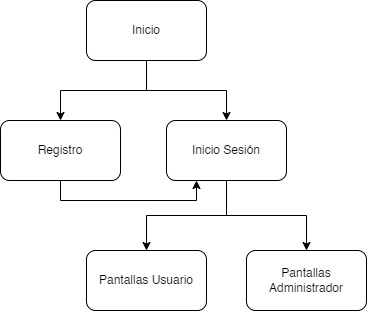
\includegraphics[width=\linewidth]{imagenes/NavegacionPrincipal.jpg}
    \caption{Navegación inicial de la aplicación}
    \label{fig:mi_imagen}
\end{figure}

\clearpage
\begin{figure}[h]
    \centering
    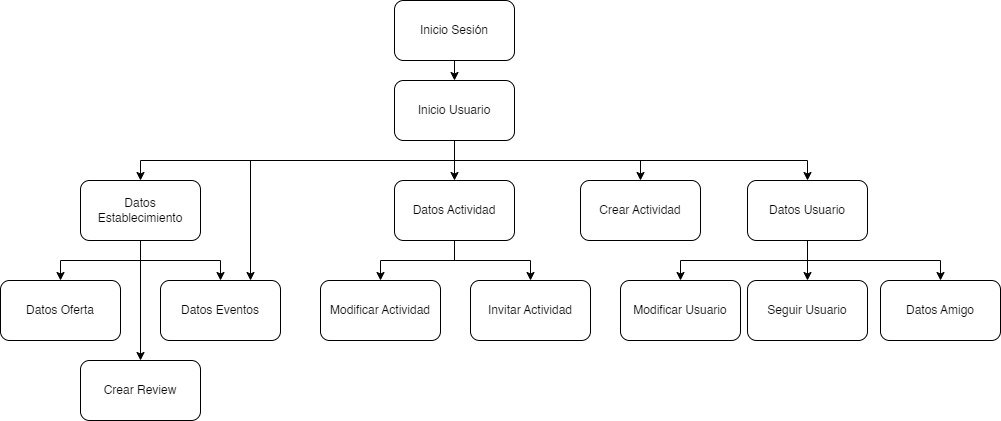
\includegraphics[width=\linewidth]{imagenes/NavegacionUsuario.jpg}
    \caption{Navegación del usuario genérico en la aplicación}
    \label{fig:mi_imagen}
\end{figure}

\clearpage
\begin{figure}[h]
    \centering
    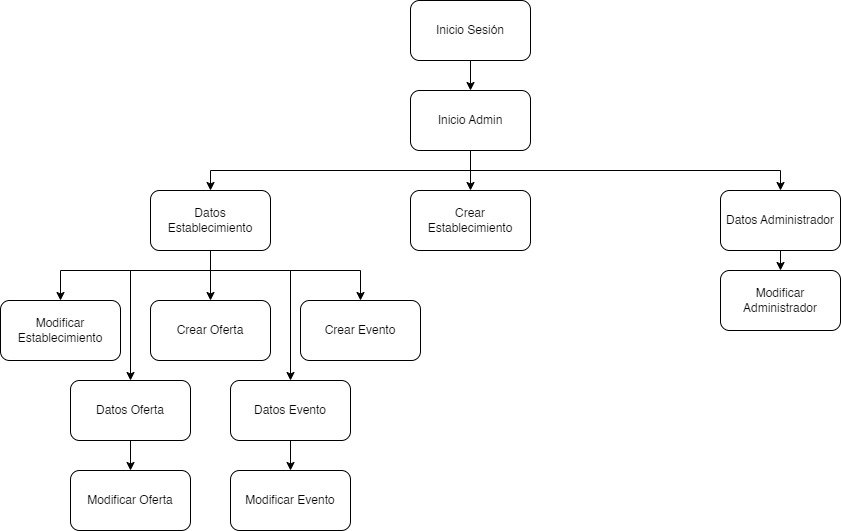
\includegraphics[width=\linewidth]{imagenes/NavegacionAdmin.jpg}
    \caption{Navegación del administrador de establecimientos en la aplicación}
    \label{fig:mi_imagen}
\end{figure}





